\documentclass[a4paper]{article}
\usepackage{amsmath}
\usepackage{hyperref}
\usepackage{pgfplots}
\pgfplotsset{compat=1.15}
\usepackage[english]{babel}

\usepackage{enumitem}
\usepackage{listings}
\usepackage{color}
\usepackage[bottom]{footmisc}

\definecolor{dkgreen}{rgb}{0,0.6,0}
\definecolor{gray}{rgb}{0.5,0.5,0.5}
\definecolor{mauve}{rgb}{0.58,0,0.82}

\lstset{frame=tb,
  language=Java,
  aboveskip=3mm,
  belowskip=3mm,
  showstringspaces=false,
  columns=flexible,
  basicstyle={\small\ttfamily},
  numbers=none,
  numberstyle=\tiny\color{gray},
  keywordstyle=\color{blue},
  commentstyle=\color{dkgreen},
  stringstyle=\color{mauve},
  breaklines=true,
  breakatwhitespace=true,
  tabsize=3
}

\begin{document}
\title{Measurement analysis of cacheability across multiple methods of grey-scaling}
\author{Niels de Waal (1698041), Jasper Smienk(1700502)}
\maketitle
\newpage

\tableofcontents
\newpage

\section{Target}
This report will focus on the cacheability of 3 different methods of grey-scaling. These will be compared to each other and the default method for grey-scaling.

These results can help decide on which algorithm to use in a facial recognition project. More and more small systems are getting an on-cpu cache. This cache should be very useful in situations where a lot of data needs to be read and processed by the cpu. Which is the case for facial recognition, where every frame needs to be read from memory and processed by the cpu. In this report, there will be an investigation using multiple methods of grey-scaling and seeing how well these methods behave with respect to the cache.

\section{Hypothesis}
We can't say anything about how they will perform against the default implementation, as we don't know how it works.

We suspect there will be very little difference between the different methods when they will be examined on their own. It is unlikely that the results will change with or without the facial recognition enabled. We do expect to see a lot of data going to the L2 cache. This because the cpu pre-fetcher should see the sequential reads from the pixel buffer and try to cache data ahead of these reads.

\section{Method}
The binary will run one of the grey-scaling methods 10000 times, and we will run this binary 10 times, after which we will aggregate the results. We will use the \textit{perf} tool for collecting the data. \textit{Perf} is a linux tool often used for measuring kernel performance. In this test we will look at both L1-dcache and L2 cache. Seeing how a single pixel is quite small in terms of the size of the data (3 * 8 bits). It could be benificial to know where most of the data ends up.

The test will be run twice for each method, once with the facial recognition, and once without.

We will make sure the tests are run on the same system and keep an eye out on the temperature to make sure it does not thermal-throttle.

Specifications of the used laptop:
\begin{center}
    \begin{tabular}{ | l | l |}
    \hline
    CPU & Intel Core i5 6600K \cite{ARK} \\ \hline
    RAM & 16GB DDR4 2400MHz \\ \hline
    OS & Linux 4.15.15-1-ARCH \\ \hline
    \end{tabular}
\end{center}

Used compiler optimisations:
\begin{itemize}[noitemsep,nolistsep]
\item -std=c++14
\item -g3
\item -ggdb
\item -g
\item -O1
\end{itemize}

Used compiler warnings:
\begin{itemize}[noitemsep,nolistsep]
\item -Wall
\item -Wextra
\item -pedantic-errors
\item -Wfatal-errors
\item -Wcast-align
\item -Wmissing-declarations
\item -Wredundant-decls
\item -Wuninitialized
\item -Wno-unused-parameter
\item -Wno-missing-field-initializers
\end{itemize}

Perf command used:
\begin{lstlisting}[language=bash]
	$ perf stat -r 10 -d -e l2_rqsts.demand_data_rd_hit,l2_rqsts.demand_data_rd_miss ./vissen}
\end{lstlisting}

\newpage
\section{Results}
\subsection{Raw data}

With facial recognition:
\begin{center}
\begin{tabular}{ |l||r|r|r|r| }
\hline
Method & L1 DCache hits & L1 DCache misses & L2 Data hits & L2 Data misses  \\
\hline\hline
Default & 209359655680 & 6524946521 & 596465950 & 50420831 \\
\hline
Averaging & 204605775027 & 5838956725 & 537926381 & 40272104 \\
\hline
Luma & 207067812232 & 5790118160 & 496829390 & 35546606 \\
\hline
Decomposition (Max)\footnotemark & - & - & - & - \\
\hline
Decomposition (Min) & 206050242309 & 5817410748 & 516984118 & 37468228 \\
\hline
\end{tabular}
\end{center}

Without facial recognition:
\begin{center}
\begin{tabular}{ |l||r|r|r|r| }
\hline
Method & L1 DCache hits & L1 DCache misses & L2 Data hits & L2 Data misses  \\
\hline\hline
Default & 20798177177 & 602197117 & 65785000 &  6469704 \\
\hline
Averaging & 13258521614 & 57533588 & 28390788 & 3701288 \\
\hline
Luma & 15789762340 & 57418201 & 28490336 &  3625812\\
\hline
Decomposition (Max) & 15789802982 & 57631568 & 28642166 & 3686989 \\
\hline
Decomposition (Min) & 15789815633 & 57681407 & 28622821 & 3807790 \\
\hline
\end{tabular}
\end{center}

\footnotetext{\texttt{Decomposistion (Max)} produced images so bad that these were unable to be used for facial recognition. This led to incorrect execution of the software, and therefore incorrect data.}

\subsection{Visualized}
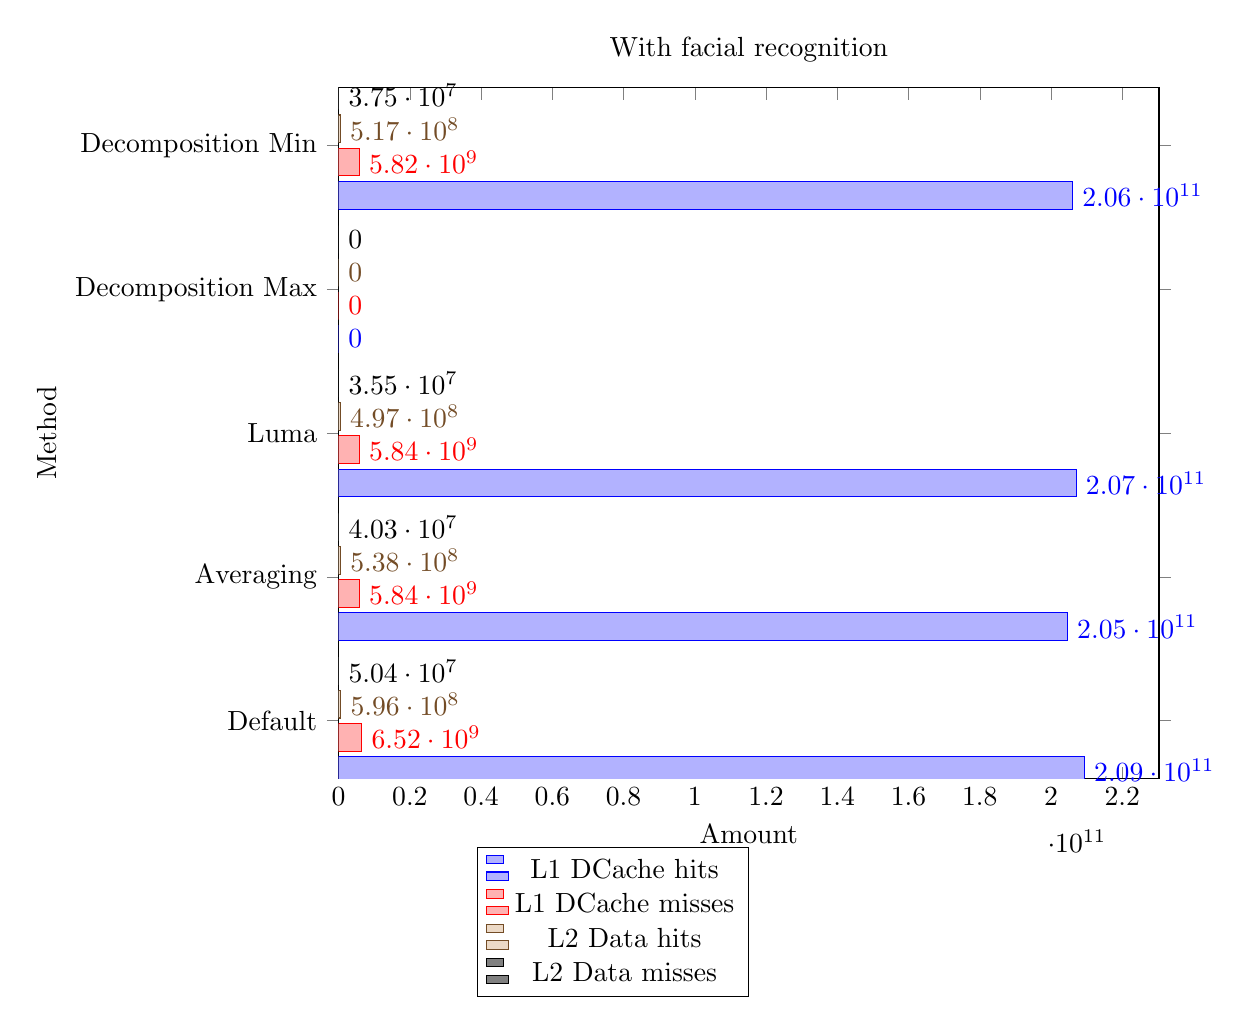
\begin{tikzpicture}
	\begin{axis}[
		title=With facial recognition,
		xbar, 
		xmin=0,
		width=12cm,
		xlabel={Amount},
		ylabel={Method},
		legend style={at={(0.5,-0.1)}},
		symbolic y coords={Default,Averaging,Luma,Decomposition Max,Decomposition Min},
		ytick=data,
		nodes near coords, nodes near coords align={horizontal},
	]
		\addplot coordinates{(209359655680,Default) (204605775027,Averaging) (207067812232,Luma) (0,Decomposition Max) (206050242309,Decomposition Min)};
		\addplot coordinates{(6524946521,Default) (5838956725,Averaging) (5838956725,Luma) (0,Decomposition Max) (5817410748,Decomposition Min)};
		\addplot coordinates{(596465950,Default) (537926381,Averaging) (496829390,Luma) (0,Decomposition Max) (516984118,Decomposition Min)};
		\addplot coordinates{(50420831,Default) (40272104,Averaging) (35546606,Luma) (0,Decomposition Max) (37468228,Decomposition Min)};
		\legend{L1 DCache hits, L1 DCache misses, L2 Data hits, L2 Data misses}
	\end{axis}
\end{tikzpicture}
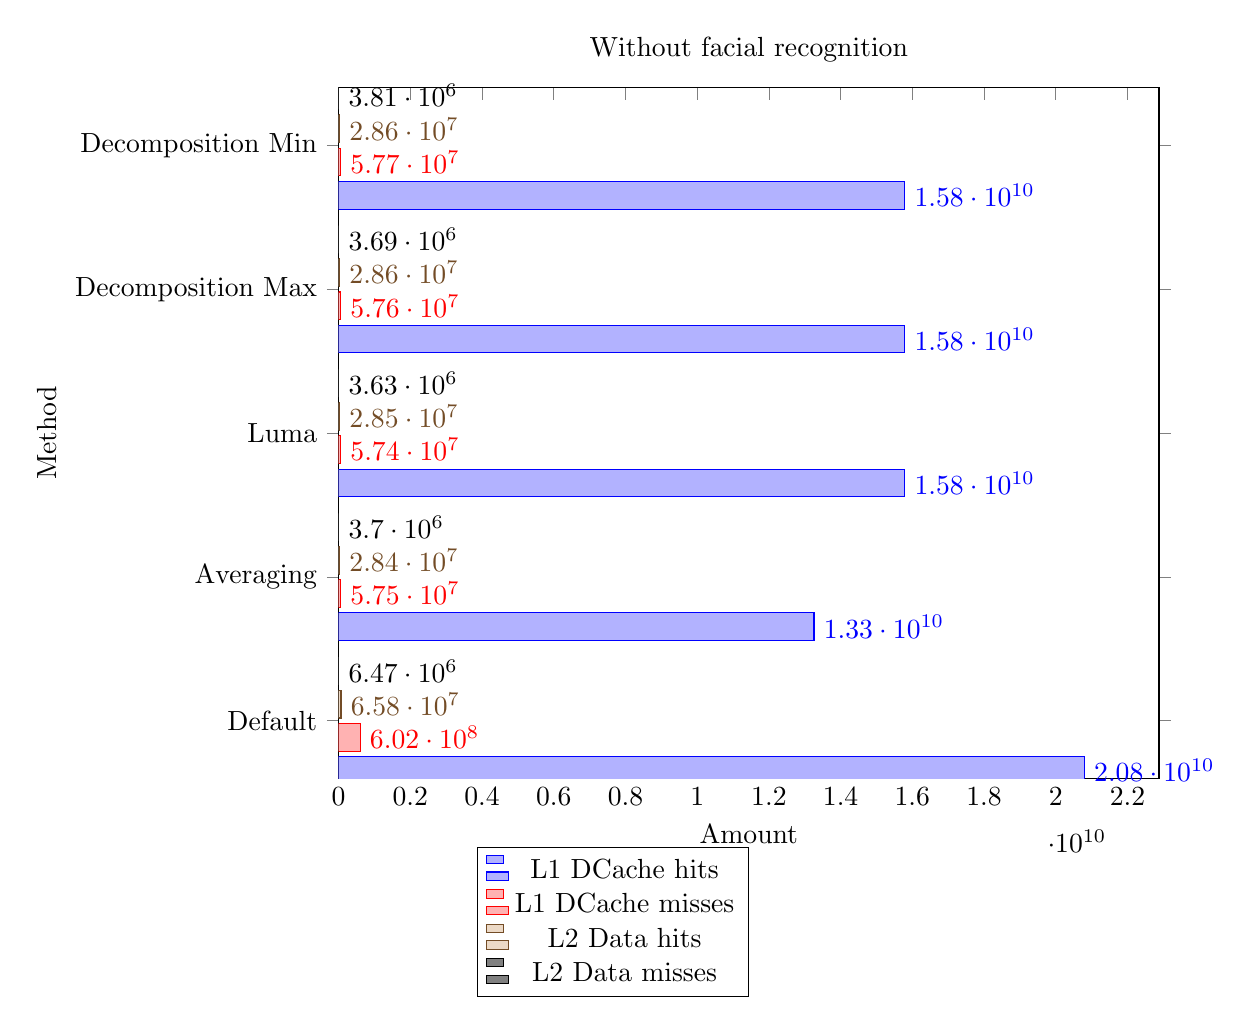
\begin{tikzpicture}
	\begin{axis}[
		title=Without facial recognition,
		xbar, 
		xmin=0,
		width=12cm,
		xlabel={Amount},
		ylabel={Method},
		legend style={at={(0.5,-0.1)}},
		symbolic y coords={Default,Averaging,Luma,Decomposition Max,Decomposition Min},
		ytick=data,
		nodes near coords, nodes near coords align={horizontal},
	]
		\addplot coordinates{(20798177177,Default) (13258521614,Averaging) (15789762340,Luma) (15789802982,Decomposition Max) (15789815633,Decomposition Min)};
		\addplot coordinates{(602197117,Default) (57533588,Averaging) (57418201,Luma) (57631568,Decomposition Max) (57681407,Decomposition Min)};
		\addplot coordinates{(65785000,Default) (28390788,Averaging) (28490336,Luma) (28642166,Decomposition Max) (28622821,Decomposition Min)};
		\addplot coordinates{(6469704,Default) (3701288,Averaging) (3625812,Luma) (3686989,Decomposition Max) (3807790,Decomposition Min)};
		\legend{L1 DCache hits, L1 DCache misses, L2 Data hits, L2 Data misses}
	\end{axis}
\end{tikzpicture}

\section{Processing}
As predicted in our hypothesis the different methods are within margin of each other. Without facial recognition, it seems that \textit{Default} has a bit more L1-DCache hits but also more L1-DCache misses.

According to our measurements it seems that both \textit{Decomposition} and \textit{Luma} perform almost identical.

\section{Conclusion}
From these measurements we can't come to a clear conclusion about a which is the better method. It seems that data from different aspects of these methods is needed to declare a winner of sorts. We can only really state that \textit{Decomposition Max} is inadvisable as it produces bad images.

\section{Evaluation}
\subsection{What went well}
The project was a very cooperative experience for both parties involved. This cooperation went very well, everyone had their tasks and did them with equal amount of dedication. This made the project an overall pleasant experience.
\subsection{What went wrong}
We both had a vigorous start with the project, however it turned out to be very hard to keep up this speed. Eventually we started to have to divide our time to other projects that required our attention at the time. This made it so we had to do a lot of work near the deadline.

Also the original plan was to use OpenCL and SIMD for parallelism. Because of the state of the relevant tools, this turned out to be quite a bit harder than was originally thought.
\subsection{What could be done differently}
A better research on the more ambitious subjects should be done in order to avoid unnecessary delays.

\begin{thebibliography}{9}

\bibitem {ARK}
	Intel
	Ark product specifications
	\url{https://ark.intel.com/products/88191/Intel-Core-i5-6600K}
	
\end{thebibliography}
\end{document}
